
\usepackage[utf8]{inputenc}
%\usepackage{ucs}
\usepackage{amsmath}
\usepackage{amsfonts}
\usepackage{amssymb}
\usepackage{multicol}
\usepackage{graphicx}
%\usepackage{hyperref}		% automatic included by beamer
\usepackage{tikz}
\usetikzlibrary{arrows,positioning,shapes}
\usepackage{listings}
\usepackage{multicol}
\usepackage{appendixnumberbeamer}
\usepackage{pstricks}
\usepackage{marvosym}
\usepackage[backend=bibtex]{biblatex}

\newcommand{\code}[1]{\texttt{#1}}

\title{perf file format}
%\subtitle{}
\author{Urs F\"assler}
\date{02.08.2011}
\institute
{
  CERN Openlab
}
%\subject{}

\lstset
{  
  basicstyle=\small\ttfamily,
  language=,
%  numbers=left,
  numberstyle={\color{Grey}},
%  identifierstyle={\color{Blue}},
%  columns=flexible,
  float=tb,
  frame=single,
  breaklines=true, % sets automatic line breaking
  breakatwhitespace=false % automatic breaks happen at whitespace
}

%\bibliographystyle{plain}
\bibliography{../report/literature}

\usetheme{Madrid}
\beamertemplatenavigationsymbolsempty

\begin{document}
\begin{frame}[plain]
  \titlepage
\end{frame}

\setcounter{framenumber}{0}

\tikzstyle{app}=[anchor=center,minimum width=3 cm,minimum height=2 cm,rectangle,rounded corners,draw=black, top color=white, bottom color=blue!30,very thick, text centered]
\tikzstyle{map}=[anchor=center,minimum width=1 cm,minimum height=1 cm,rectangle,rounded corners,very thick, text centered,draw=black,fill=white]
\tikzstyle{event}=[map, fill=green!30,very thick, text centered]
\tikzstyle{arrow}=[->,thick]
\tikzstyle{Interface}=[rectangle,draw=black, fill=yellow!60,rotate=90]
\tikzstyle{file}=[anchor=center,draw=black, top color=white, bottom color=yellow!30,thick, text centered]

\begin{frame}{initialization}
\begin{center}
\begin{tikzpicture}[scale=0.9,transform shape]

\path [thick, dotted] (0,-4) edge (0,4);
\node [anchor=east] at (0,3.5) ()  {Kernelspace};
\node [anchor=west] at (0,3.5) ()  {Userspace};


\node [app] at (-4,0) (linux)  {Linux};
\node [app,minimum width=3 cm,minimum height=2 cm] at (4,0) (perf)  {perf record};

\visible<2>{
  \path [arrow,bend right=10] (perf) edge (linux);
}

\node [Interface] at (0,0) (iface) {perf\_event};

\node  [anchor=center,minimum width=1 cm,minimum height=2 cm,rectangle,draw=black, top color=white, bottom color=yellow!30,thick, text centered] at ( 6, -3) (file) {file};
\visible<2>{
  \path [arrow,bend right=-20] (perf) edge (file);
}
\end{tikzpicture}
\end{center}
\end{frame}

\begin{frame}{recording}
\begin{center}
\begin{tikzpicture}[scale=0.9,transform shape]
\path [thick, dotted] (0,-4) edge (0,4);
\node [anchor=east] at (0,3.5) ()  {Kernelspace};
\node [anchor=west] at (0,3.5) ()  {Userspace};
\node [Interface,minimum width=6 cm] at (0,0) (iface) {mmap};

\node [app] at (-4,0) (linux)  {Linux};
\node [app,minimum width=3 cm,minimum height=2 cm] at (4,0) (perf)  {perf record};

\visible<3->{
  \path [arrow,bend right=-15] (linux) edge node[above]{signal} (perf);
}

\visible<2->{
\node  [event] at (-2,-2) (ev0) {\tiny{sample}};
\node  [event] at (-1,-2) (ev1) {\tiny{sample}};
\node  [event] at ( 0,-2) (ev2) {\tiny{lost}};
\node  [event] at ( 1,-2) (ev3) {\tiny{comm}};
\node  [event] at ( 2,-2) (ev4) {\tiny{sample}};

\path [arrow,bend right=30] (linux) edge (ev0);
\path [arrow,bend right=30] (ev4) edge (perf);

\node  [map] at ( 0, 2) (ev5) {};
\node  [map] at (-1, 2) (ev6) {};
\node  [map] at (-2, 2) (ev7) {};

\path [arrow,bend right=20] (perf) edge (ev5);
\path [arrow,bend right=30] (ev7) edge (linux);
}

\node [file,minimum width=1 cm,minimum height=2 cm,rectangle] at ( 6, -3) (file) {file};
\visible<3->{
  \path [arrow,bend right=-20] (perf) edge (file);
}
\end{tikzpicture}
\end{center}
\end{frame}

\begin{frame}{perf file format\only<handout>{ (simplified, see page \ref{sec:fileformat})}}
\begin{center}
\begin{tikzpicture}[scale=0.9,transform shape]

\node [file,rectangle split, rectangle split parts=4] at (-4,0) (header){
  \textbf{file\_header}
  \nodepart{second} attr
  \nodepart{third} data
  \nodepart{fourth} ...
};

\visible<2->{
\node [file,rectangle split, rectangle split parts=3] at (0,2) (fileattr0){
  \textbf{file\_attr}
  \nodepart{second} ''cycles''
  \nodepart{third} ...
};
\node [file,rectangle split, rectangle split parts=3] at (4,2) (fileattr1){
  \textbf{file\_attr}
  \nodepart{second} ''instructions''
  \nodepart{third} ...
};
\path [arrow,bend right=10] (header) edge (fileattr0.south);
\path [arrow] (fileattr0) edge (fileattr1);
}

\visible<3->{
\node [event,rectangle split, rectangle split parts=4] at (-1,-2) (ev0){
  sample
  \nodepart{second} period
  \nodepart{third} ip\only<handout>{\footnote{instruction pointer}}
  \nodepart{fourth} ...
};

\node [event,rectangle split, rectangle split parts=4] at (2,-2) (ev1){
  mmap\only<handout>{\footnote{not the same as on the previous slide}}
  \nodepart{second} memory range
  \nodepart{third} filename
  \nodepart{fourth} ...
};

\node [event,rectangle split, rectangle split parts=4] at (5,-2) (ev2){
  sample
  \nodepart{second} period
  \nodepart{third} ip
  \nodepart{fourth} ...
};

\node [event,rectangle split, rectangle split parts=4] at (7,-2) (ev3){
  sample
  \nodepart{second} period
  \nodepart{third} ip
  \nodepart{fourth} ...
};

\path [arrow,bend right=-5] (header) edge (ev0.north);
\path [arrow] (ev0) edge (ev1);
\path [arrow] (ev1) edge (ev2);
\path [arrow] (ev2) edge (ev3);
}

\visible<4>{
  \path [arrow,dotted] (ev0.north) edge (fileattr0.south);
  \path [arrow,dotted] (ev2.north) edge (fileattr1.south);
  \path [arrow,dotted] (ev3.north) edge (fileattr0.south);
}

\visible<5>{
  \path [arrow,dotted,bend right=30] (ev0.south) edge (ev1.south);
  \path [arrow,dotted,bend left=30] (ev2.south) edge (ev1.south);
  \path [arrow,dotted,bend left=30] (ev3.south) edge (ev1.south);
}
\end{tikzpicture}
\end{center}
\end{frame}

\begin{frame}{Demo}
\only<handout>{
  \rput[lt](0.5,3){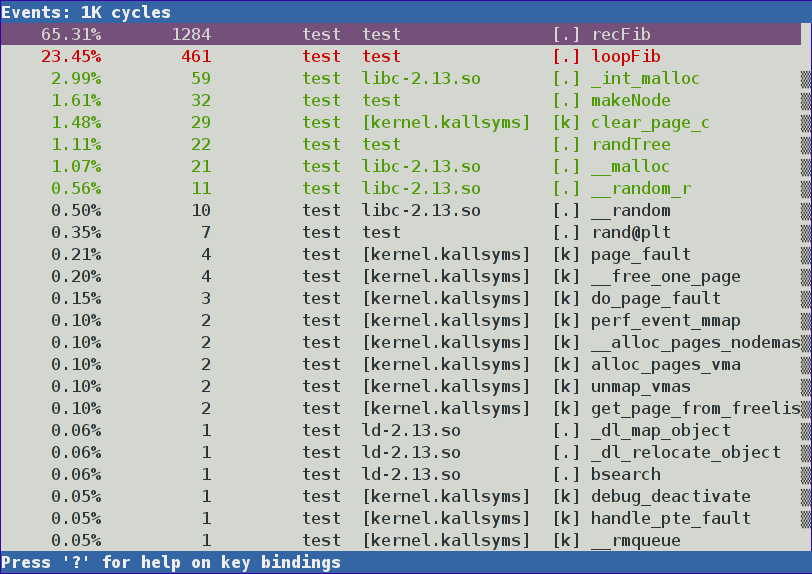
\includegraphics[width=11cm]{res/perfReport}}
  \rput[lt](3,0.5){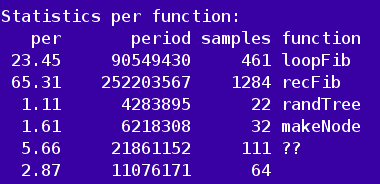
\includegraphics[width=6cm]{res/readperf}}
}
\end{frame}

\begin{frame}{detailed file format\label{sec:fileformat}}
\centering{
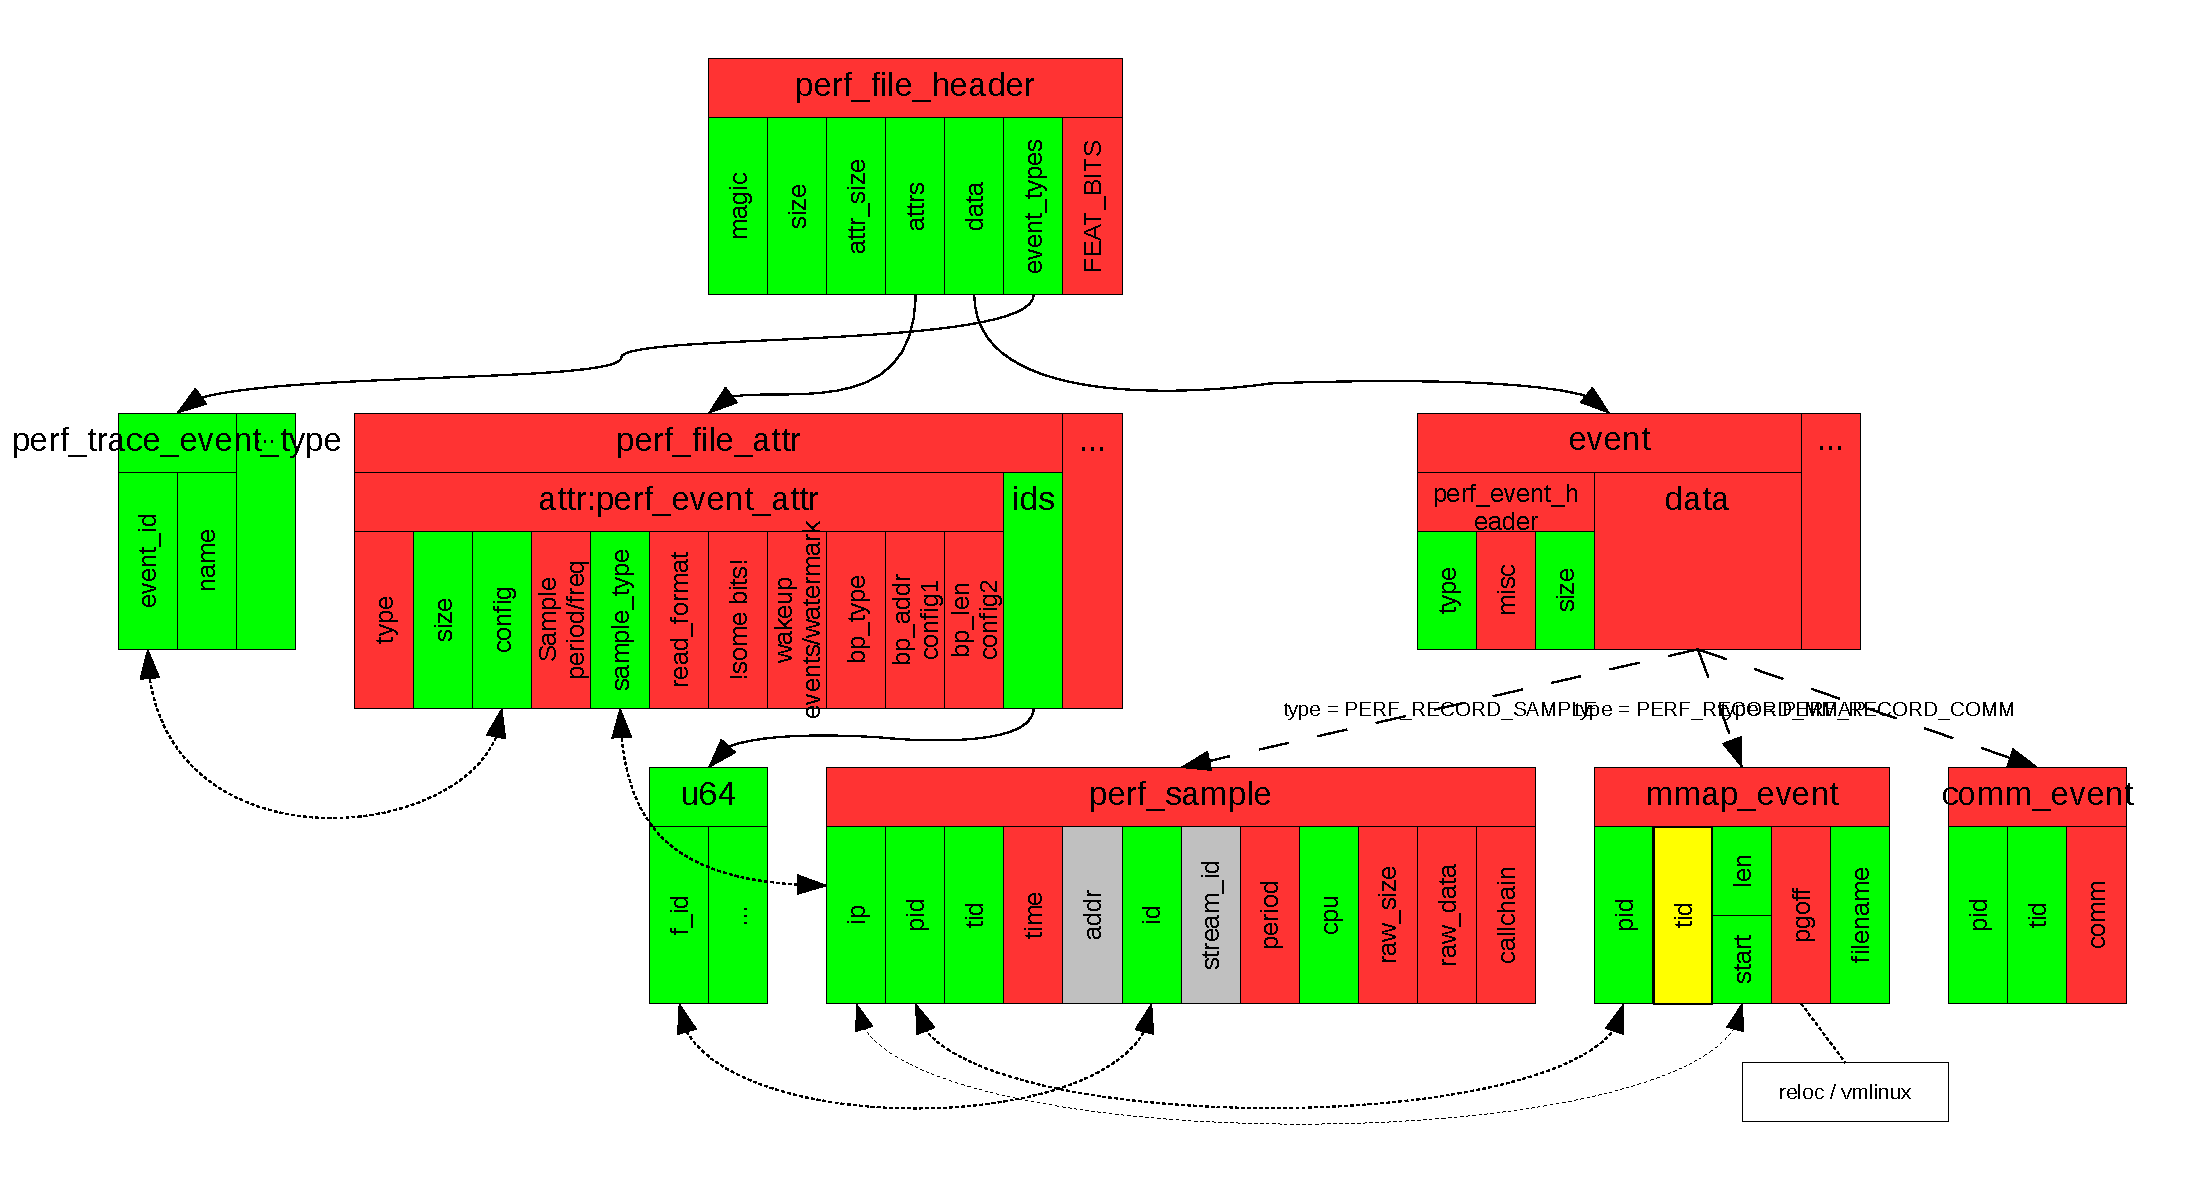
\includegraphics[width=12cm]{res/fileformat}
}
\end{frame}

\begin{frame}{map ip to function name}
\begin{enumerate}
  \item sample contains Instruction Pointer
  \item find corresponding mmap event\only<handout>{\footnote{IP has to be in range of mmap}}
  \begin{itemize}
    \item mmap events contains binary name
  \end{itemize}
  \item addr2line shows source file and function name from IP and binary
  \item aggregate all samples in the same function
\end{enumerate}
\end{frame}

\begin{frame}{further work}
\begin{itemize}
  \item understand timestamp of sample
  \item mapping instruction pointer to library functions
%  \item understand mapping event names $\leftrightarrow$ hex code
  \item understand how the address $\leftrightarrow$ filename works
\end{itemize}
\end{frame}

\begin{frame}{summary}
\begin{itemize}
  \item good understanding of file format
  \begin{itemize}
    \item map samples to functions
    \item same result as perf report
    \item library and system function doesn't work entirely
  \end{itemize}
\end{itemize}
\end{frame}

\only<handout>{
\appendix
\section{Appendix}

\begin{frame}{Analyze virtualized machine}
\code{perf} has support for the Kernel-based Virtual Machine (KVM \cite{kvm}). For the performance measurement, an argument tells \code{perf} that the machine using KVM should be monitored. It uses the PMU of the host. It seems that also detailed information is available if the host machine has access to the guests \code{/proc/} files. Measures of hardware counters from inside the virtual machine is not supported.

VirtualBox \cite{virtualbox} is not supported. This has two consequences. First, \code{perf} on the host can not record data about the guest. Second, there is no PMU in the virtual machine and therefore \code{perf} can not record hardware counters.
\end{frame}

\only<handout>{
\begin{frame}{literature}
\begin{scriptsize}
  \printbibliography
\end{scriptsize}
\end{frame}
}

}

\end{document}
